\documentclass[12pt,a4paper]{article}
\usepackage[utf8]{inputenc}
\usepackage{amsmath}
\usepackage{amsfonts}
\usepackage{amssymb}
\usepackage[brazil]{babel}
\usepackage{indentfirst}
\usepackage{url}
\usepackage{float}
\usepackage{color}
\usepackage{setspace}
%%%%%%%%%%Codigos para o JAVA%%%%%%%%%%%%%%%%%%%%%%%%%%%%%%%%
\definecolor{pblue}{rgb}{0.13,0.13,1}
\definecolor{pgreen}{rgb}{0,0.5,0}
\definecolor{pred}{rgb}{0.9,0,0}
\definecolor{pgrey}{rgb}{0.46,0.45,0.48}
\usepackage{listings}
\lstset{language=Java,
  showspaces=false,
  showtabs=false,
  breaklines=true,
  showstringspaces=false,
  breakatwhitespace=true,
  commentstyle=\color{pgreen},
  keywordstyle=\color{pblue},
  stringstyle=\color{pred},
  basicstyle=\ttfamily,
  moredelim=[il][\textcolor{pgrey}]{\$\$},
  moredelim=[is][\textcolor{pgrey}]{\%\%}{\%\%}
}
%%%%%%%%%%%%%%%%%%%%%%%%%%%%%%%%Fim codigo JAVA%%%%%%%%%%%%%%
%%%%%%%%%%%Codigo geral%%%%%%%%%%%%%%%%%%%%%%%%%%%%%%%%%%%%%%
\definecolor{mygreen}{rgb}{0,0.6,0}
\definecolor{mygray}{rgb}{0.5,0.5,0.5}
\definecolor{mymauve}{rgb}{0.58,0,0.82}
\lstset{ %
  backgroundcolor=\color{white},   % choose the background color; you must add \usepackage{color} or \usepackage{xcolor}; should come as last argument
  basicstyle=\footnotesize,        % the size of the fonts that are used for the code
  breakatwhitespace=false,         % sets if automatic breaks should only happen at whitespace
  breaklines=true,                 % sets automatic line breaking
  captionpos=b,                    % sets the caption-position to bottom
  commentstyle=\color{mygreen},    % comment style
  deletekeywords={...},            % if you want to delete keywords from the given language
  escapeinside={\%*}{*)},          % if you want to add LaTeX within your code
  extendedchars=true,              % lets you use non-ASCII characters; for 8-bits encodings only, does not work with UTF-8
  frame=single,                    % adds a frame around the code
  keepspaces=true,                 % keeps spaces in text, useful for keeping indentation of code (possibly needs columns=flexible)
  keywordstyle=\color{blue},       % keyword style
  language=Octave,                 % the language of the code
  morekeywords={*,...},            % if you want to add more keywords to the set
  numbers=left,                    % where to put the line-numbers; possible values are (none, left, right)
  numbersep=5pt,                   % how far the line-numbers are from the code
  numberstyle=\tiny\color{mygray}, % the style that is used for the line-numbers
  rulecolor=\color{black},         % if not set, the frame-color may be changed on line-breaks within not-black text (e.g. comments (green here))
  showspaces=false,                % show spaces everywhere adding particular underscores; it overrides 'showstringspaces'
  showstringspaces=false,          % underline spaces within strings only
  showtabs=false,                  % show tabs within strings adding particular underscores
  stepnumber=1,                    % the step between two line-numbers. If it's 1, each line will be numbered
  stringstyle=\color{mymauve},     % string literal style
  tabsize=2,                       % sets default tabsize to 2 spaces
  title=\lstname                   % show the filename of files included with \lstinputlisting; also try caption instead of title
}
%%%%%%%%%%%%%%%%%%%%%%%%%%%%%%%%Fim codigo geral%%%%%%%%%%%%%
\RequirePackage{graphicx}
\title{JDBC com transações}
\author{Daniel Moreira Cardoso \and Gusttavo Nunes Gomes\and Jeferson Rossini Ferreira Lourenço\and Paulo Henrique Rodrigues Araujo\and Warley Rodrigues de Andrade}
 
\usepackage[left=3cm,right=3cm,top=2cm,bottom=2cm]{geometry}
\begin{document}
\begin{titlepage}
\begin{center}
\begin{figure}[htb]
                
                \label{figura:LogoIF}
        
                \centering
                \includegraphics[width=6cm]{recursos/imagens/logo.png} 
\end{figure}
Instituto Federal Goiano - Campus Ceres\\
Bacharelado em Sistemas de Informação\\
Prof. Me. Ronneesley Moura Teles\\\vspace{0.5cm}
Jonathan Silvestre\\
Fernando Maciel\\
Warley Rodrigues\\
\vspace{5.0cm}
\textit{\textbf{\Large{Introdução a JSF}}}\\\vspace{0.5cm}
\vspace{9.5cm}
\end{center}
\end{titlepage}
\tableofcontents
\newpage
\begin{center}
\textbf{\Large{Introdução a JSF}}\\\vspace{0.5cm}
\end{center}

\section{Introdução}
JavaServer Faces ou apenas JSF, é um framework que permite a criação de interfaces de usuário web colocando componentes visuais pré-prontos, de forma que o desenvolvedor não se preocupe com Javascript e HTML. Basta adicionarmos os componentes (calendários, tabelas, formulários) e eles serão renderizados e exibidos em formato html. Seu ponto forte é um grande número de componentes e um design muito flexível o que fez com que esse Framework crescesse muito abordando novas tecnologias.

Desenvolvido pela comunidade JCP (Java Community Process), atualmente o JSF é o framework preferido para o desenvolvimento de aplicações Web possuindo um excelente conjunto de funcionalidades para o cenário de desenvolvimento em que é inserido, possibilitando ao programador preocupar-se somente com a lógica de negócio deixando as tarefas básicas e trabalhosas por conta do framework.

\subsection{O JavaSecer Faces possui as seguintes partes}
\begin{itemize}
\item Conjunto de componentes pré-fabricados de Interface de Usuário (IU);

\item Modelo de programação orientado a eventos;

\item Modelo de componentes que permite a desenvolvedores independentes fornecerem componentes adicionais.
\end{itemize}

\subsection{Característica marcante}
\begin{itemize}
\item Entidades e regras de negócio;

\item Objetos gerais da aplicação (dados, etc.)
Visão;

\item Componentes UI em páginas JSP/XHTML;

\item Kits renderizadores (HTML, WML, XML, etc.)
Controlador;

\item Faces Servlet (Front Controller);

\item Backing Bean (Page Controller ou Modelo).
\end{itemize}

\subsection{Principais motivos que levaram JFS ao sucesso}
\begin{itemize}
\item Ser uma especificação EE (Enterprise Edition)  desde da 5ª Versão;

\item Ser um framework cuja a API foi pensada no trabalho dos desenvolvedores de IDEs;

\item Possuir comunidades ativas em fóruns, assim facilitando a procura sobre duvidas e sugestões;

\item Exigir baixo conhecimento inicial para criação de interfaces de usuários tradicionais;

\item Possuir ótimas bibliotecas de componentes livres e pagas desenvolvidas por terceiros;

\item Possuir Ajax nativo em sua versão 2.0.
\end{itemize}

A aplicação Desktop é um tipo de aplicação que é instalada no computador local e acessa o banco de dados ou gerenciador de arquivos, para o uso de sua aplicação é utilizado Delphi, VB (Visual Basic) ou, no mundo Java, Swing. Ela possui componentes para cada tipo de sistema um desenvolvimento rico possuindo calendários, menus diversos ou componentes drag and drop (arrastar e soltar).

\section{Principais provedores do projeto JSF}
\subsection{Mojorra}
A tecnologia JavaServer Faces simplifica a criação de interfaces de usuário para aplicativos JavaServer. Os desenvolvedores podem criar aplicativos da Web montando componentes de UI reutilizáveis em uma página, conectando esses componentes a uma fonte de dados do aplicativo e fiação de eventos gerados pelo cliente para manipulando os eventos do lado do servidor. Este projeto fornece informações sobre o desenvolvimento contínuo da especificação JavaServer Faces.

\subsection{MyFaces}
O Apache MyFaces é um projeto da Apache Software Foundation e hospeda vários subprojetos relacionados à tecnologia JavaServer fornecendo tecnologias como:
\begin{itemize}
\item Implementação JavaServer (MyFaces Core, providing api/impl and bundle modules);

\item Várias bibliotecas de componentes que contêm widgets UI para construir web-applications com JSF (MyFaces Tomahawk, MyFaces Trinidad, MyFaces Tobago);

\item Patoces de extensão para JavaServer (MyFaces Orchestra, MyFaces Extensions Validator, MyFaces Extensions CDI);

\item Módulos de integração para outras tecnologias e padrões (MyFaces Portlet Bridge for integration with the portlet-standard).
\end{itemize}

\subsection{ADF}
O Oracle ADF é uma estrutura de Java EE de ponta a ponta que simplifica o desenvolvimento de aplicativos, fornecendo serviços de infraestrutura prontos e uma experiência de desenvolvimento visual e declarativa.

ADF Model: permite uma abordagem unificada para vincular qualquer interface de usuário a qualquer serviço de negócio, sem a necessidade de escrever código. É o principal módulo do framework.

\textbf{Ele oferece:}
\begin{itemize}
\item ADF Business Components: simplifica a construção de serviços de negócio;

\item ADF Faces rich client: possui uma grande variedade de componentes de interface AJAX para aplicações JSF;

\item ADF Controller: integra o JSF com o ADF Model. É uma extensão do JSF Controller com várias funcionalidades adicionais, como as Task Flows.
\end{itemize}

\section{Componentes do projeto JSF}
\subsection{RichFaces}
O projeto RichFaces é uma estrutura avançada de componentes de interface do usuário para integrar facilmente os recursos do Ajax em aplicativos de negócios usando o JSF, sua última atualização o RichFaces 4 baseia-se no suporte pioneiro do Ajax que começou com o RichFaces 3 e está padronizado no JSF 2.

Além de ampliar esses recursos do ajax, o RichFaces também melhora outras áreas do JSF 2, incluindo usabilidade, ajuste de desempenho, recursos dinâmicos, esfoliante e componente desenvolvimento. Isso permite aos usuários tirar o máximo proveito de todos os aprimoramentos de produtividade do JSF 2. 

\textbf{Disponibilizando:}
\begin{itemize}
\item Um conjunto completo de componentes habilitados para o AJAX em duas bibliotecas a a4j que tem seus controles centralizados da AJAX e a Rico que componentes autônomos e prontos para usar;

\item Validação do lado do cliente, expandindo a validação de feixe JSR 303 até o navegador;
\item Encaminhamento avançado para combinar os requisitos de alto desempenho das aplicações empresariais do mundo real;

\item Atualizações de componentes de envio, incluindo integrações do Serviço JavaMessaging (JMS) e vários mecanismos de transporte baseados no suporte do navegador;

\item Possui o próprio kit de desenvolvimento de componentes (CDK);

\item Documentação abrangente que aloca as melhores práticas de desenvolvimento e os detalhes dos componentes;

\item Detalhadas e automatizados testes instalações de componentes, ações, ouvintes e páginas;

\item Suporte abrangente para o navegador cruzado;

\item Comunidade grande e ativa em sua fundação.
\end{itemize}

\subsection{PrimeFaces}
A Prime Technology não é um fornecedor de software, mas uma casa de desenvolvimento de software junto com as atividades de consultoria e treinamento. Uma estrutura que nem sequer é usada por seus próprios criadores pode facilmente perder pontos vitais em termos de usabilidade e simplicidade, uma diferença importante em comparação com os produtos do fornecedor é que em todos os projetos de seus clientes o PrimeFaces é usado como o framework de front-end. Isso ajuda a visualizar o projeto do ponto de vista do desenvolvedor de aplicativos para que possa facilmente perceber os recursos perdidos e corrigir rapidamente os erros diferindo significativamente o PrimeFaces de outras bibliotecas.

\subsection{OpenFaces}
O OpenFace é uma implementação Python e Torch do reconhecimento facial com redes neurais profundas e é baseado no documento CVPR 2015 FaceNet, consiste em uma Incorporação Unificada para Reconhecimento de Rosto e Clustering por Florian Schroff, Dmitry Kalenichenko e James Philbin no Google. A tocha permite que a rede seja executada em uma CPU ou com CUDA. 

\textbf{Concedendo:}
\begin{itemize}
\item Detecção rostos com modelos pré-treinados de dlib ou OpenCV;

\item Transforma o rosto em códigos mandando para a rede neural;

\item Usando uma rede neural profunda para representar (ou incorporar) o rosto em uma hiperesfera de unidade de 128 unidades. A incorporação é uma representação genérica para o rosto de qualquer pessoa. Ao contrário de outras representações do rosto, essa incorporação tem a propriedade agradável de que uma distância maior entre dois embutidos de rosto significa que os rostos provavelmente não são da mesma pessoa. Esta propriedade torna as tarefas de agrupamento, similaridade de detecção e classificação mais fáceis do que outras técnicas de reconhecimento facial, onde a distância euclidiana entre recursos não é significativa;

\item Aplica várias técnicas de classificação ou agrupamento preferenciais para os recursos para completar sua tarefa de reconhecimento;
\end{itemize}

\subsection{IceFaces}
O ICEfaces é um framework de desenvolvimento de aplicativos Rich Internet (RIA) de código aberto para Java EE. O ICEfaces funciona em plataformas que vão desde desktops a telefones inteligentes e Apple para Android. Ele melhora a eficiência do desenvolvedor, enquanto reduz o tempo ao mercado e os custos operacionais. São recursos e recursos ricos que permitem aos desenvolvedores fazer mais dentro dos limites de uma infraestrutura herdada do que pode ser imaginada.
 
\vspace{0.5cm}
\textbf{Ela oferece escopos com várias formas de se trabalhar em um projeto como:}

\subsubsection{Automatic Ajax}
O ICEfaces inclui vários recursos inovadores, como envio único, renderização direta para DOM e atualizações parciais de página que resultam cumulativamente no Ajax automático, eliminando completamente a necessidade de os desenvolvedores transmitirem as atualizações de página usando as tags padrão JSF <f: ajax>;

\subsubsection{Ajax Push}
A colaboração em tempo real é suportada no ICEfaces através dos mecanismos Ajax Push , o que facilita o envio assíncrono de atualizações de página para navegadores de clientes sem a necessidade de uma apresentação iniciada pelo usuário. Isso significa que os usuários do aplicativo podem ser informados instantaneamente sempre que ocorrer uma alteração de estado no aplicativo.

\subsubsection{Resource Management}
O ICEfaces amplia o framework JSF para auxiliar no gerenciamento de recursos. ICEfaces inclui novas anotações para ajustar o comportamento dos beans View-scoped. Embora o escopo View seja uma adição bem-vinda para gerenciar o ciclo de vida dos beans, o comportamento do escopo View pode não ser intuitivo em certos cenários. Especificamente, as anotações permitem que você controle o comportamento dos feixes de escala de visualização em navegação repetida para a mesma exibição e durante a exibição de disposição;

\subsubsection{Scoped Resource Registry}
O ResourceRegistry permite que um aplicativo registre instâncias javax.faces.application.Resource em tempo de execução. Cada Recurso está registrado em um escopo especificado (Aplicativo, Sessão, Vista, Flash ou Janela) para que o recurso possa ser coletado por lixo quando o escopo expirar;

\subsubsection{Streamlined Configuration}
O JSF 2 simplifica a configuração alavancando as anotações e os ICEfaces estão em conformidade com esta estratégia, simplificando a configuração em várias áreas. Os servlets específicos de ICEfaces e muitos dos parâmetros de configuração no ICEfaces 1.x não são mais necessários com ICEfaces. Isso torna ainda mais rápido e fácil adicionar ICEfaces ao seu aplicativo JSF e reduz consideravelmente a possibilidade de perda de produtividade devido a pequenos erros de configuração.

\subsubsection{Window Scope}
O ICEfaces apresenta um novo escopo personalizado chamado Window Scope, que é projetado para preencher uma lacuna nos escopos existentes disponíveis para o JSF 2, como ele existe para a vida de uma janela ou guia do navegador, incluindo sobreviver recarrega e atualiza.

\subsection{EasyFaces}
http://www.easyfaces.com.br 

\subsection{Gmaps4jsf}
Ele visa integrar mapas do Google com o JSF. Os usuários do JSF também serão capazes de construir Panoramas e mapas complexos do Streetview com apenas algumas linhas de código (tags JSF). GMaps4JSF é uma das bibliotecas JSF Mashups que permite que os usuários do JSF criem aplicativos de mashup da Web 2.0 no JSF facilmente.

Ele permite manipular mapas como criações de mapa usando (latitude e longitude) ou (endereço), adicione marcadores, adicionar textos de informações, adicionar controles, desenhar polígonos, polilinhas e círculos, eventos nos objetos, adicionar groundOverlay, executar operações diferentes, alterar entre tipos de mapas e etc.

\section{Extensões JSF}
\subsection{PrettyFaces}
O PrettyFaces é uma biblioteca open source de reescrita de URLs que facilita criação de URLs amigáveis (Friendly URLs), tornando suas páginas mais acessíveis para os usuários, possuindo um mecanismos que facilita a chamada de métodos através da URL no JSF.

\subsection{OmniFaces}
É uma biblioteca de utilitários que busca facilitar o desenvolvimento JSF para aplicações corporativas. Foi criada por Bauke Scholtz (BalusC) e Arjan Tijms, colaboradores regulares no popular site Stack Overflow de perguntas e respostas. Ele complementa as bibliotecas JSF existentes com várias classes auxiliares e soluções para problemas específicos. A amostra de componentes no site de demonstração do OmniFaces (live showcase), por exemplo, é baseada no PrimeFaces. 

\textbf{Ele oferece:}
\begin{itemize}
\item Destaca os campos que falharam na validação;

\item Importação de valores de constantes para dentro do escopo da EL (Expression Language);

\item Conversão automática de objetos do modelo em drop-downs e outros componentes de seleção;

\item Valida todos os campos para valores como “todos ou nenhum”, “todos iguais”, “um ou mais” e “em ordem”, além de validações de “valor único”;

\item RenderKit HTML5, que adiciona suporte a diversos atributos específicos do HTML5 para componentes UIForm e UIInput;

\item Manipuladores de exceção Ajax: uma página de erro será exibida quando uma exceção ocorrer durante uma solicitação Ajax do JSF;

\item Árvore com código de marcação personalizado por nível (utilizável para vários casos de uso recursivos);

\item Coleções de funções da EL para lidar com arrays, conversões, datas e strings;

\item Filtro de compressão GZIP para respostas HTTP;

\item Funcionalidades para inclusão de Servlets e páginas JSP no Facelets.

\end{itemize}

\section{Referências Bibliográfica}
\noindent 
Listagem de frameworks Java. Acesso em: 09 de novembro de 2017. Disponìvel em: \url {https://imasters.com.br/linguagens/java/listagem-de-frameworks-java/?trace=1519021197&source=single}
\\
\\\vspace{0.2cm}
O que é JSF ?. Acesso em: 09 de novembro de 2017. Diponível em: \url{https://fernandogodoy.wordpress.com/2011/02/12/o-que-e-jsf/}

\end{document}
%Modelo de código para inserir figura
%\begin{figure}[h]
%\centering
%\includegraphics[width=15cm]{logo.png}
%\label{4}
%\caption{Fonte:http://...; Acesso em 06/11/2017}
%\end{figure}
